


\begin{markdown}
#### Add tasks
The task Group is default.

Enter the task Title.
Enter the task description in the Description.
Switch the toggle button to Flag this task?.
Select the Due date.
Click Save and add another, to add another task.
Click Confirm.
\end{markdown}

\begin{figure}[H]
    \centering
    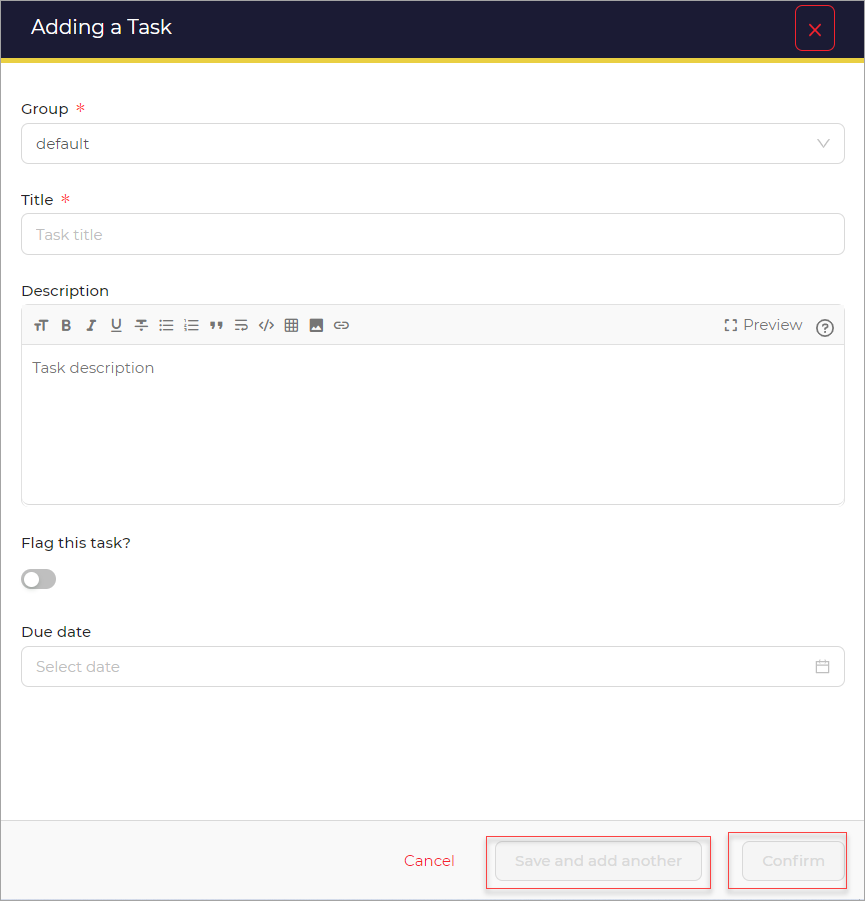
\includegraphics[width=\textwidth]{images/docs/analyst/cases/addition/adding_a_task.png}
    \caption{add a task}
    \label{fig:modules}
\end{figure}

\begin{markdown}

#### Add tags
Choose tags from the Taxonomy. The selected tag will appear in the Selected Tags box.
Click the Add selected tags button.
\end{markdown}



\begin{figure}[H]
    \centering
    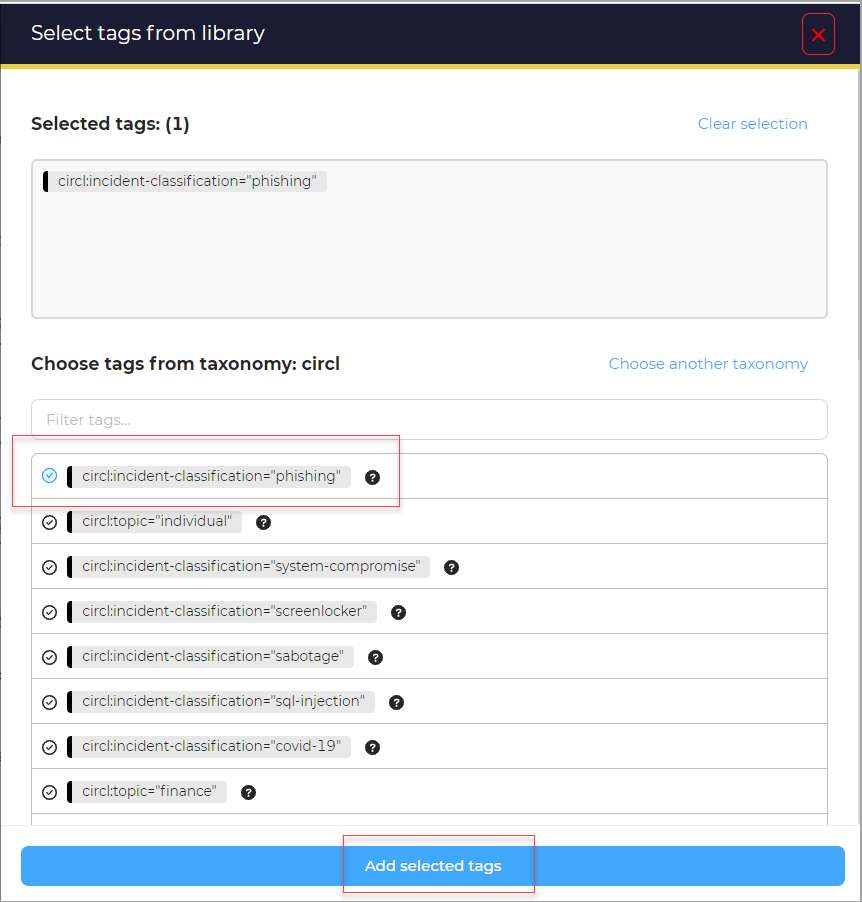
\includegraphics[width=\textwidth]{images/docs/analyst/cases/addition/select_tags.png}
    \caption{add tags}
    \label{fig:modules}
\end{figure}
\begin{markdown}

#### Add pages
By selecting Create new page
Enter the page Title.
Enter or select the Category.
Enter the page content in the content.
Click Confirm.
Click Save and add another, to add another task.
\end{markdown}



\begin{figure}[H]
    \centering
    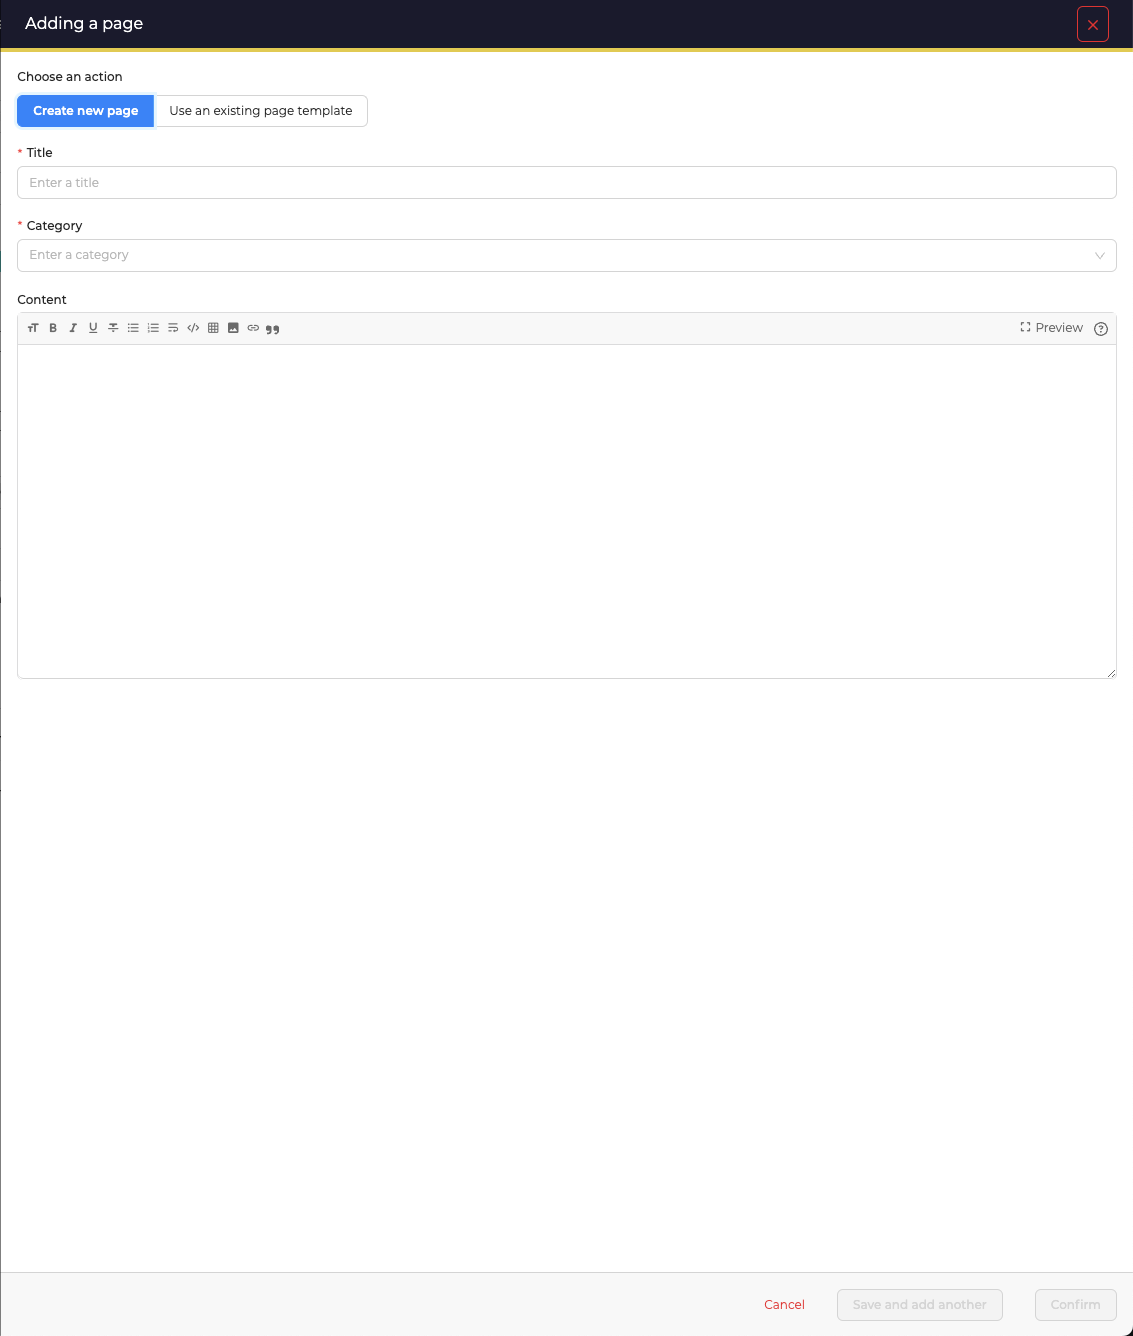
\includegraphics[width=\textwidth]{images/docs/analyst/cases/addition/adding_a_new_page.png}
    \caption{add a new page}
    \label{fig:modules}
\end{figure}

By selecting Use an existing page template

Choose template(s) from those available in the list of existing templates
Click Confirm.
Click Save and add another, to add another task.

\begin{figure}[H]
    \centering
    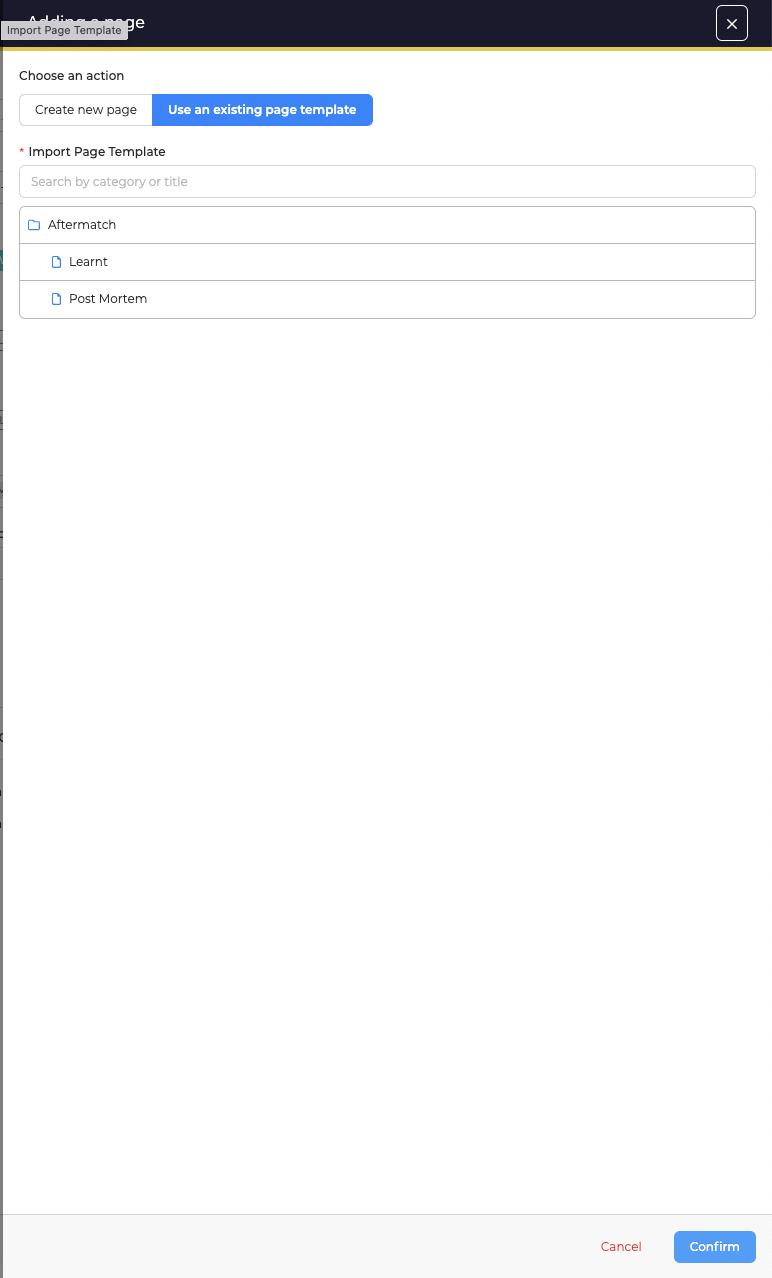
\includegraphics[width=\textwidth]{images/docs/analyst/cases/addition/adding_a_existng_page.png}
    \caption{with an existing page}
    \label{fig:modules}
\end{figure}